%% LyX 2.3.0 created this file.  For more info, see http://www.lyx.org/.
%% Do not edit unless you really know what you are doing.
\documentclass[english,showpacs,preprintnumbers,amssymb,aps,notitlepage,twocolumn]{revtex4-1}
\usepackage{lmodern}
\renewcommand{\sfdefault}{lmss}
\renewcommand{\ttdefault}{lmtt}
\usepackage[T1]{fontenc}
\usepackage[latin9]{inputenc}
\setcounter{secnumdepth}{3}
\usepackage{color}
\usepackage{array}
\usepackage{multirow}

\makeatletter

%%%%%%%%%%%%%%%%%%%%%%%%%%%%%% LyX specific LaTeX commands.
%% Binom macro for standard LaTeX users
\newcommand{\binom}[2]{{#1 \choose #2}}

%% Because html converters don't know tabularnewline
\providecommand{\tabularnewline}{\\}

%%%%%%%%%%%%%%%%%%%%%%%%%%%%%% User specified LaTeX commands.
\usepackage{amsfonts,amsmath} % amsmath added here instead to prevent clash with lyx function
% this is the preamble created by tikzit, we can edit this in the final document to change the shapes we use for nodes, edge styles, etc... 
% just be sure to use the same name for the same kind of node/edge in any figures you make


\usepackage[svgnames]{xcolor}
\usepackage{tikz}
\usetikzlibrary{decorations.markings}
\usetikzlibrary{shapes.geometric}
%\pagestyle{empty}

\newcommand\scaledLW{0.5} % scaled linewidth for fig 2, defined globally so they can be changed easily

\newcommand\scaledNodeSize{0.5} % scaled node size for fig 2, defined globally so they can be changed easily

\pgfdeclarelayer{edgelayer}
\pgfdeclarelayer{nodelayer}
\pgfsetlayers{edgelayer,nodelayer,main}

\tikzstyle{none}=[inner sep=0pt]

\tikzstyle{rn}=[circle,fill=Red,draw=Black,line width=0.8 pt]
\tikzstyle{gn}=[circle,fill=Lime,draw=Black,line width=0.8 pt]
\tikzstyle{yn}=[circle,fill=Yellow,draw=Black,line width=0.8 pt]
\tikzstyle{auxiliary_qubit}=[circle,fill=Red,draw=Black,scale=0.8]
\tikzstyle{logical_qubit}=[circle,fill=Black,draw=Black,scale=0.8]
\tikzstyle{emb_logical_qubit}=[circle,fill=Gray,draw=Black,scale=0.8,line width=2.000]
\tikzstyle{emb_auxiliary_qubit}=[circle,fill=Red,draw=Black,scale=0.8,line width=2.000]
\tikzstyle{unused_qubit}=[circle,fill=Gray,draw=Gray,scale=0.8]
\tikzstyle{arrow_end}=[circle,fill=none,draw=none,scale=.1]




\tikzstyle{simple}=[-,draw=Black,line width=1.000]
\tikzstyle{added}=[-,draw=Black,line width=1.000]
%\tikzstyle{added}=[-,draw=green,line width=1.000]
\definecolor{tempcolor}{rgb}{.9,.9,.9}
\tikzstyle{unused}=[-,draw=tempcolor,line width=0.500]
%\definecolor{tempcolor}{rgb}{.7,.9,.7}
%\tikzstyle{unused_added}=[-,draw=tempcolor,line width=1.000]
%\tikzstyle{unused_added}=[-,draw=green,draw opacity=1,line width=1.000,dashed]
%\tikzstyle{unused_added}=[-,draw=cyan,draw opacity=1,line width=0.5]
\tikzstyle{unused_added}=[-,draw=gray,draw opacity=1,line width=0.5]
\tikzstyle{embedding}=[-,draw=Black,line width=3.000]
\tikzstyle{arrow}=[-,draw=Black,postaction={decorate},decoration={markings,mark=at position .5 with {\arrow{>}}},line width=2.000]



\newcommand{\intextheight}{13 pt}

\@ifundefined{showcaptionsetup}{}{%
 \PassOptionsToPackage{caption=false}{subfig}}
\usepackage{subfig}
\makeatother

\usepackage{babel}
\begin{document}

\title{Embedding quadratization gadgets on Chimera and Pegasus graphs}

\author{Nike Dattani}
\email{n.dattani@cfa.harvard.edu}

\selectlanguage{english}%

\affiliation{Harvard-Smithsonian Center for Astrophysics}

\author{Nicholas Chancellor}
\email{nicholas.chancellor@durham.ac.uk}

\selectlanguage{english}%

\affiliation{Durham University}
\begin{abstract}
We group all known quadratizations of cubic and quartic binary optimization
problems into five and seven unique graphs respectively. We then perform
a minor embedding of these graphs onto the well-known Chimera graph,
and the brand new \emph{Pegasus} graph. In cases where two or more
graphs have a minor embedding with the same overhead in terms of auxiliary
variables, we make recommendations for which gadgets are best to use
for certain problems. 
\end{abstract}
\maketitle
Discrete optimization problems are often naturally formulated in terms
of minimizing some polynomial of degree $>2$, which is then `quadratized'
into a quadratic function which can be solved using standard algorithms
for universal classical computers {[}1{]}, using special-purpose classical
annealers {[}2{]}, or using quantum annealers {[}3{]}. With dozens
of quadratization methods available {[}4{]}, one should choose the
best quadratization for a given problem, and for a given method for
solving the problem. 

\noindent 
\begin{figure*}
\caption{\label{fig:allGraphGadgets}}

\newcommand{\thisfigheight}{1.5 cm}

\subfloat[``\emph{all to aux}'']{

\resizebox{!}{\thisfigheight}{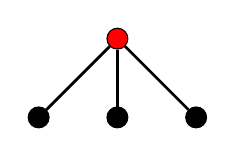
\begin{tikzpicture}
	\begin{pgfonlayer}{nodelayer}
		\node [style=auxiliary_qubit] (0) at (0, 5) {};
		\node [style=logical_qubit] (1) at (-1, 4) {};
		\node [style=logical_qubit] (2) at (0, 4) {};
		\node [style=logical_qubit] (3) at (1, 4) {};
	\end{pgfonlayer}
	\begin{pgfonlayer}{edgelayer}
		\draw [style=simple] (1) to (0);
		\draw [style=simple] (0) to (2);
		\draw [style=simple] (0) to (3);
	\end{pgfonlayer}
\end{tikzpicture}
}}\subfloat[``\emph{Y}'']{

\resizebox{!}{\thisfigheight}{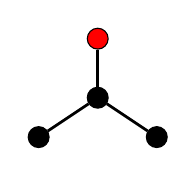
\begin{tikzpicture}
	\begin{pgfonlayer}{nodelayer}
		\node [style=logical_qubit] (0) at (0, -0) {};
		\node [style=auxiliary_qubit] (1) at (0, 0.75) {};
		\node [style=logical_qubit] (2) at (0.75, -0.5) {};
		\node [style=logical_qubit] (3) at (-0.75, -0.5) {};
	\end{pgfonlayer}
	\begin{pgfonlayer}{edgelayer}
		\draw [style=simple] (2) to (0);
		\draw [style=simple] (3) to (0);
		\draw [style=simple] (1) to (0);
	\end{pgfonlayer}
\end{tikzpicture}
 }}\subfloat[\mbox{``\emph{coat hanger}''}]{

\resizebox{!}{\thisfigheight}{\input{tikzit/k4_missing_2edge.tikz}
}}\subfloat[]{

\resizebox{!}{\thisfigheight}{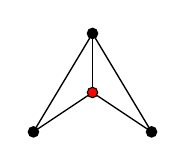
\begin{tikzpicture}[every node/.style={scale=\scaledNodeSize}]
	\begin{pgfonlayer}{nodelayer}
		\node [style=auxiliary_qubit] (0) at (0, -0) {};
		\node [style=logical_qubit] (1) at (0, 0.75) {};
		\node [style=logical_qubit] (2) at (0.75, -0.5) {};
		\node [style=logical_qubit] (3) at (-0.75, -0.5) {};
	\end{pgfonlayer}
	\begin{pgfonlayer}{edgelayer}
		\draw [style=simple,line width=\scaledLW] (3) to (1);
		\draw [style=simple,line width=\scaledLW] (1) to (2);
		\draw [style=simple,line width=\scaledLW] (2) to (0);
		\draw [style=simple,line width=\scaledLW] (3) to (0);
		\draw [style=simple,line width=\scaledLW] (1) to (0);
	\end{pgfonlayer}
\end{tikzpicture}

}}\subfloat[``\emph{all to all}'']{

\resizebox{!}{\thisfigheight}{\input{tikzit/k4.tikz}}}

\subfloat[\emph{``all to aux''}]{

\resizebox{!}{\thisfigheight}{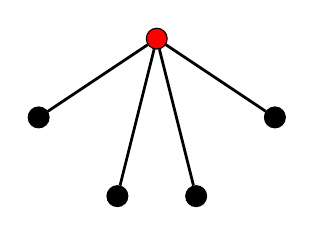
\begin{tikzpicture}
	\begin{pgfonlayer}{nodelayer}
		\node [style=logical_qubit] (0) at (-1, -0) {};
		\node [style=logical_qubit] (1) at (0, -1) {};
		\node [style=logical_qubit] (2) at (1, -1) {};
		\node [style=logical_qubit] (3) at (2, -0) {};
		\node [style=auxiliary_qubit] (4) at (0.5, 1) {};
	\end{pgfonlayer}
	\begin{pgfonlayer}{edgelayer}
		\draw [style=simple] (0) to (4);
		\draw [style=simple] (1) to (4);
		\draw [style=simple] (2) to (4);
		\draw [style=simple] (4) to (3);
	\end{pgfonlayer}
\end{tikzpicture}
}}\subfloat[``\emph{tripod}'']{

\resizebox{!}{\thisfigheight}{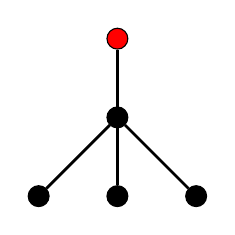
\begin{tikzpicture}
	\begin{pgfonlayer}{nodelayer}
		\node [style=logical_qubit] (0) at (0, -0) {};
		\node [style=auxiliary_qubit] (1) at (0, 1) {};
		\node [style=logical_qubit] (2) at (-1, -1) {};
		\node [style=logical_qubit] (3) at (1, -1) {};
		\node [style=logical_qubit] (4) at (0, -1) {};
	\end{pgfonlayer}
	\begin{pgfonlayer}{edgelayer}
		\draw [style=simple] (1) to (0);
		\draw [style=simple] (2) to (0);
		\draw [style=simple] (3) to (0);
		\draw [style=simple] (4) to (0);
	\end{pgfonlayer}
\end{tikzpicture}
}}\subfloat[``\emph{all to two aux + 1}'']{\resizebox{!}{\thisfigheight}{\input{tikzit/2aux_to_all4_1conn.tikz}}}\subfloat[``\emph{all to all - 1}'']{

\resizebox{!}{\thisfigheight}{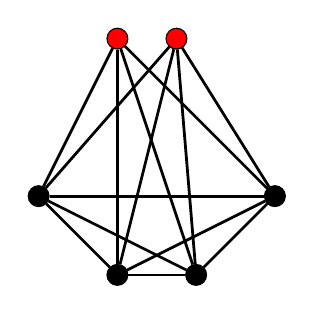
\begin{tikzpicture}
	\begin{pgfonlayer}{nodelayer}
		\node [style=logical_qubit] (0) at (-1, -0) {};
		\node [style=logical_qubit] (1) at (2, -0) {};
		\node [style=auxiliary_qubit] (2) at (0, 2) {};
		\node [style=auxiliary_qubit] (3) at (0.75, 2) {};
		\node [style=logical_qubit] (4) at (0, -1) {};
		\node [style=logical_qubit] (5) at (1, -1) {};
	\end{pgfonlayer}
	\begin{pgfonlayer}{edgelayer}
		\draw [style=simple] (2) to (1);
		\draw [style=simple] (0) to (3);
		\draw [style=simple] (3) to (1);
		\draw [style=simple] (4) to (1);
		\draw [style=simple] (0) to (2);
		\draw [style=simple] (5) to (3);
		\draw [style=simple] (5) to (4);
		\draw [style=simple] (5) to (2);
		\draw [style=simple] (5) to (1);
		\draw [style=simple] (4) to (3);
		\draw [style=simple] (4) to (2);
		\draw [style=simple] (4) to (0);
		\draw [style=simple] (0) to (5);
		\draw [style=simple] (0) to (1);
	\end{pgfonlayer}
\end{tikzpicture}

}}\subfloat[``\emph{all to aux + $K_{4}$}'']{ 

\resizebox{!}{\thisfigheight}{\input{tikzit/2auxConn_to_all4_allConn.tikz}}}\subfloat[``\emph{all to aux} again'']{

\resizebox{!}{\thisfigheight}{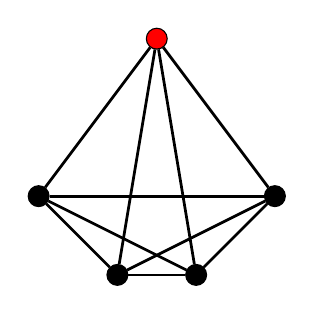
\begin{tikzpicture}
	\begin{pgfonlayer}{nodelayer}
		\node [style=logical_qubit] (0) at (2, -0) {};
		\node [style=auxiliary_qubit] (1) at (0.5, 2) {};
		\node [style=logical_qubit] (2) at (0, -1) {};
		\node [style=logical_qubit] (3) at (-1, -0) {};
		\node [style=logical_qubit] (4) at (1, -1) {};
	\end{pgfonlayer}
	\begin{pgfonlayer}{edgelayer}
		\draw [style=simple] (1) to (0);
		\draw [style=simple] (2) to (0);
		\draw [style=simple] (3) to (0);
		\draw [style=simple] (4) to (2);
		\draw [style=simple] (4) to (3);
		\draw [style=simple] (4) to (1);
		\draw [style=simple] (4) to (0);
		\draw [style=simple] (2) to (3);
		\draw [style=simple] (3) to (1);
		\draw [style=simple] (2) to (1);
	\end{pgfonlayer}
\end{tikzpicture}
}}\subfloat[``\emph{two $K_{4}'s$}'']{

\resizebox{!}{\thisfigheight}{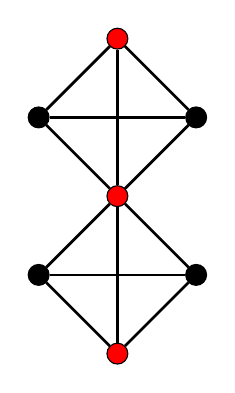
\begin{tikzpicture}
	\begin{pgfonlayer}{nodelayer}
		\node [style=logical_qubit] (0) at (-1, -0) {};
		\node [style=auxiliary_qubit] (1) at (0, 3) {};
		\node [style=logical_qubit] (2) at (-1, 2) {};
		\node [style=auxiliary_qubit] (3) at (0, 1) {};
		\node [style=logical_qubit] (4) at (1, -0) {};
		\node [style=auxiliary_qubit] (5) at (0, -1) {};
		\node [style=logical_qubit] (6) at (1, 2) {};
	\end{pgfonlayer}
	\begin{pgfonlayer}{edgelayer}
		\draw [style=simple] (2) to (1);
		\draw [style=simple] (3) to (1);
		\draw [style=simple] (4) to (0);
		\draw [style=simple] (0) to (5);
		\draw [style=simple] (4) to (5);
		\draw [style=simple] (6) to (3);
		\draw [style=simple] (6) to (2);
		\draw [style=simple] (6) to (1);
		\draw [style=simple] (2) to (3);
		\draw [style=simple] (0) to (3);
		\draw [style=simple] (4) to (3);
		\draw [style=simple] (5) to (3);
	\end{pgfonlayer}
\end{tikzpicture}
}}
\end{figure*}

There are ways to quadratize functions of discrete variables without
adding any auxiliary variables {[}5{]}, but when those methods cannot
be applied we introduce auxiliary variables. The resulting quadratic
functions (called `gadgets') that accurately or exactly simulate the
original high-degree functions, will have some connectivity between
the binary variables (or bits, or qubits, herein referred to for convenience
only as qubits) which can be represented by a graph in which vertices
represent qubits and edges indicate when two different qubits appear
together in a quadratic term. Since this graph incorporates no information
about the linear terms, constant term, or the coefficients of the
quadratic terms, many different gadgets have the same graph, therefore
in this paper we will classify all known quadratization gadgets into
categories according to their corresponding graph (herein called their
`gadget graph'). 

Gadget graphs for all known single cubic terms and for all known single
quartic terms are given in Figure \ref{fig:allGraphGadgets}. Gadget
graphs tell us a lot about how costly the quadratic optimization problem
will be, and those with larger connectivity tend to yield more difficult
functions to optimize. Furthermore, some optimization methods only
work if their corresponding graph has a certain connectivity, two
examples of such connectivities being the ones in D-Wave's well-known
Chimera graph {[}5{]}, and in their very recently presented \emph{Pegasus}
graph, both shown in Fig. \ref{fig:ChimeraAndPegasus}.

\begin{table}[b]
\caption{}

\rule{1\columnwidth}{0.5pt}

\begin{tabular*}{1\columnwidth}{@{\extracolsep{\fill}}ccccc}
\hline 
\noalign{\vskip2mm}
\multirow{2}{*}{{\footnotesize{}Gadget Graph}} & \multirow{2}{*}{{\footnotesize{}Example Gadgets}} & {\footnotesize{}$N_{{\rm aux}}$} & {\footnotesize{}$N_{{\rm aux}}$ } & {\footnotesize{}$N_{{\rm aux}}$ }\tabularnewline
 &  & {\scriptsize{}Quadratization} & {\scriptsize{}Chimera} & {\scriptsize{}Pegasus}\tabularnewline[2mm]
\hline 
\noalign{\vskip2mm}
\multicolumn{5}{c}{Cubic $\rightarrow$ Quadratic}\tabularnewline[2mm]
\hline 
\noalign{\vskip2mm}
\multirow{2}{*}{\textbf{\textcolor{blue}{\scriptsize{}All to Aux}}} & {\scriptsize{}NTR-KZFD} & \multirow{2}{*}{{\scriptsize{}1}} & \multirow{2}{*}{{\scriptsize{}0}} & \multirow{2}{*}{{\scriptsize{}0}}\tabularnewline
 & {\scriptsize{}NTR-ABCG} &  &  & \tabularnewline[0.5mm]
\textbf{\textcolor{blue}{\scriptsize{}Y}} & {\scriptsize{}NTR-ABCB} & {\scriptsize{}1} & {\scriptsize{}0} & {\scriptsize{}0}\tabularnewline[0.5mm]
\textbf{\textcolor{blue}{\scriptsize{}Coat Hanger}} & {\scriptsize{}AR} & {\scriptsize{}1} & {\scriptsize{}1} & {\scriptsize{}0}\tabularnewline[0.5mm]
\textbf{\textcolor{blue}{\scriptsize{}(d)}} & {\scriptsize{}ACR} & {\scriptsize{}1} &  & {\scriptsize{}0}\tabularnewline[0.5mm]
\multirow{3}{*}{\textbf{\textcolor{blue}{\scriptsize{}All to All}}} & {\scriptsize{}PTR-Ishikawa} & \multirow{3}{*}{{\scriptsize{}1}} & \multirow{3}{*}{} & \multirow{3}{*}{{\scriptsize{}0}}\tabularnewline
 & {\scriptsize{}PTR-BCR(1-4)} &  &  & \tabularnewline
 & {\scriptsize{}PTR-KZ} &  &  & \tabularnewline[2mm]
\hline 
\noalign{\vskip2mm}
\multicolumn{5}{c}{{\scriptsize{}Quartic $\rightarrow$ Quadratic}}\tabularnewline[2mm]
\hline 
\noalign{\vskip2mm}
\textbf{\textcolor{blue}{\scriptsize{}All2Aux}} & {\scriptsize{}NTR-KZFD} & {\scriptsize{}1} & {\scriptsize{}0} & {\scriptsize{}0}\tabularnewline
\textbf{\textcolor{blue}{\scriptsize{}Tripod}} & {\scriptsize{}NTR-ABCB} & {\scriptsize{}1} & {\scriptsize{}0} & {\scriptsize{}0}\tabularnewline
\textbf{\textcolor{blue}{\scriptsize{}All22Aux+1}} & {\scriptsize{}PTR} & {\scriptsize{}2} & {\scriptsize{}1} & {\scriptsize{}0}\tabularnewline
\textbf{\textcolor{blue}{\scriptsize{}All2All - 1}} & {\scriptsize{}PTR-Ishikawa} & {\scriptsize{}2} & {\scriptsize{}?} & {\scriptsize{}2}\tabularnewline
\multirow{2}{*}{\textbf{\textcolor{blue}{\scriptsize{}All2Aux+$K_{4}$}}} & {\scriptsize{}PTR-BCR-2} & \multirow{2}{*}{{\scriptsize{}1}} & \multirow{2}{*}{{\scriptsize{}3}} & \multirow{2}{*}{{\scriptsize{}2}}\tabularnewline
 & {\scriptsize{}PTR-BCR-4} &  &  & \tabularnewline
\textbf{\textcolor{blue}{\scriptsize{}All2Aux}} & {\scriptsize{}PTR-BCR-3} & {\scriptsize{}2} & {\scriptsize{}?} & {\scriptsize{}2}\tabularnewline
\textbf{\textcolor{blue}{\scriptsize{}Two $K_{4}'s$}} & {\scriptsize{}PTR-KZ} & {\scriptsize{}3} & {\scriptsize{}?} & {\scriptsize{}1}\tabularnewline[2mm]
\hline 
\end{tabular*}

\rule{1\columnwidth}{0.5pt}
\end{table}

\begin{figure}
\caption{\label{fig:ChimeraAndPegasus}}
\end{figure}

Any graph, can be mapped onto the Chimera or Pegasus graphs by minor-embedding
{[}6{]}, where the Chimera graph or the Pegasus graph is a graph minor
of the graph representing the problem that needs to be optimized.
This often means that one binary variable in the quadratic optimization
problem needs to be represented by two qubits instead of one, making
the number of qubits needed to solve the original problem much larger
than before, and sometimes completely impossible. For example a quartic
function with 1000 binary variables has $\binom{1000}{3}>166$ million
possible cubic terms and $\binom{1000}{4}>40$ billion possible quartic
terms which have to be quadratized, and then minor-embedded. If our
minimization method can only be applied for up to 50 billion qubits,
we cannot afford for each quartic-to-quadratic gadget to require its
own auxiliary qubit for minor-embedding.

We have provided minor-embeddings for all gadget graphs in Figure
\ref{fig:allGraphGadgets}, for both Chimera and Pegasus. We note
that \textbf{\emph{all}} cubic to quadratic gadgets involvnig one
auxiliary qubit can be embedded onto Pegasus without any further auxiliary
qubits for the embedding, because Pegasus contains the $K_{4}$ graph,
which means any possible connections between the three logical qubits
and the one auxiliary qubit are already contained in Pegasus. Since
Chimera does not contain $K_{4}$, only negative cubic terms are so
far known to be quadratizable with gadgets that embed directly onto
Chimera without any extra qubits for the embedding.

\section{Minor embeddings for cubic to quadratic gadgets}

\subsection{Chimera graph}

\begin{figure*}
\caption{Minor embeddings of all cubic to quadratic gadgets onto a `unit cell'
of a Chimera graph. Transparent vertices and edges are not used. Thick
black edges denote graph minors, in which two physical qubits (two
vertices) represent one logical qubit (this is done when logical qubits
need to be connected to more qubits than the Chimera unit cell otherwise
allows).}

\newcommand{\chimeraFigSize}{3cm}

\subfloat[``\emph{all to aux''}]{\resizebox{!}{\chimeraFigSize}{\input{tikzit/all_to_aux_chimera.tikz}}}\subfloat[``\emph{Y''}]{\resizebox{!}{\chimeraFigSize}{\input{tikzit/logical_fork_chimera.tikz}}}\subfloat[``\emph{coat hanger''}]{\resizebox{!}{\chimeraFigSize}{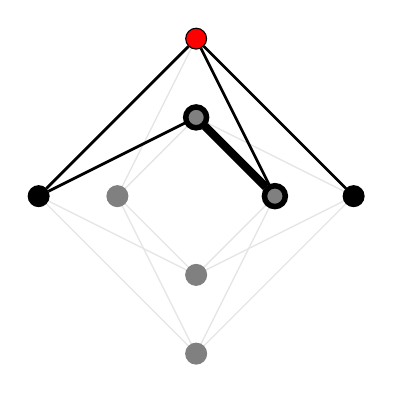
\begin{tikzpicture}
	\begin{pgfonlayer}{nodelayer}
		\node [style={logical_qubit}] (0) at (-2, 0) {};
		\node [style={unused_qubit}] (1) at (-1, 0) {};
		\node [style={logical_qubit}] (2) at (2, 0) {};
		\node [style={emb_logical_qubit}] (3) at (0, 1) {};
		\node [style={unused_qubit}] (4) at (0, -1) {};
		\node [style={unused_qubit}] (5) at (0, -2) {};
		\node [style={emb_logical_qubit}] (6) at (1, 0) {};
		\node [style={auxiliary_qubit}] (7) at (0, 2) {};
	\end{pgfonlayer}
	\begin{pgfonlayer}{edgelayer}
		\draw [style=unused] (1) to (3);
		\draw [style=unused] (3) to (2);
		\draw [style=unused] (1) to (4);
		\draw [style=unused] (4) to (2);
		\draw [style=unused] (4) to (0);
		\draw [style=unused] (0) to (5);
		\draw [style=unused] (5) to (2);
		\draw [style=unused] (5) to (1);
		\draw [style=embedding] (6) to (3);
		\draw [style=unused] (6) to (4);
		\draw [style=unused] (6) to (5);
		\draw [style=simple] (0) to (7);
		\draw [style=simple] (6) to (7);
		\draw [style=simple] (7) to (2);
		\draw [style=unused] (1) to (7);
		\draw [style=simple] (0) to (3);
	\end{pgfonlayer}
\end{tikzpicture}
}}\subfloat[``\emph{''}]{\resizebox{!}{\chimeraFigSize}{\input{tikzit/k4_missing_edge_chimera.tikz}}}\subfloat[``\emph{all to all''}]{\resizebox{!}{\chimeraFigSize}{\input{tikzit/k4_chimera.tikz}}}

\end{figure*}


\end{document}
